\documentclass[a4j,12pt,dvipdfmx]{jreport}

%%%%%%%%%%%%%%%%%%%%%%%%%%%%%%%%%%%%%%%%%%%%%%%%%%%%%%%%%%%%%%%
% 1. texの冒頭に\usepackage{NGC}と記述してください.
%
% 2. 文字列の色替えをキャンセルしたい(文字を黒くしたい)場合は,
%    NGC.styの中身を編集してください.
%    編集手順はNGC.styに書いてあります.
%%%%%%%%%%%%%%%%%%%%%%%%%%%%%%%%%%%%%%%%%%%%%%%%%%%%%%%%%%%%%%%

\usepackage{NGC}
\usepackage{algorithmic,algorithm}
\usepackage{amsmath}
\usepackage{amssymb}
\usepackage{amsthm}
\usepackage{bm}
\usepackage{graphicx}
\usepackage{todonotes}
\usepackage{url}

% 図・表がページ全体を占めても良い割合を少し増やす
\renewcommand{\topfraction}{0.7} % 上部で占める最大の割合
\renewcommand{\bottomfraction}{0.7} % 下部で占める最大の割合
\renewcommand{\textfraction}{0.3} % テキストが占める最小割合
\renewcommand{\floatpagefraction}{0.7} % 単独になるときの最小割合

\renewcommand{\arraystretch}{.9}

\title{組み合わせ回路における\\信頼性の効率的計算手法}
\author{津島 雅俊}
\stdnum{6611130040-3}
\date{\today}

\begin{document}

\maketitle

\newpage
\thispagestyle{empty}
\pagenumbering{roman}
\setcounter{page}{1}
\chapter*{内容梗概}


%It has been anticipated that a so-called "soft error"
%causes serious problems even in a combinatorial logic circuits consisting of the near-future generation of transistors.
近い将来,トランジスタによって構成される組み合わせ回路では,
動作中に発生する可能性のあるソフトエラーが深刻な問題となることが予想されている.
%Thus it is very important to develop efficient methods for the reliability analysis of logic circuits.
したがって,論理回路の信頼性を効率的に評価する手法の開発は,
回路の設計において非常に重要となってきている.

%There is an efficient reliability analysis method based on Probabilistic Transfer Matrix (PTM),
論理回路の信頼性を評価するための既存の手法としては,Probabilistic Transfer Matrix (PTM) を用いた手法が存在する.
%but the necessary peak memory would be very huge in the worst case.
しかし,この手法は,最悪の場合,非常に大きなメモリが必要となる.
%This paper proposes another approach that uses much less memory even in the worst case.
そこで,本研究では,既存手法とは異なるアプローチを用いてメモリの使用量を削減する.
%Our method carefully considers to avoid essentially the same computation
%as much as possible to reduce the computational time.
\cyannout{このアルゴリズムは,各入力に対して出力が正しく得られる確率を用いて,ゲート数に比例した空間計算量で計算する.
計算途中に発生する同じ計算を減らすことによって,計算時間を減らす工夫も行われている.}

%Our preliminary experimental results show that the memory usage would be less than a ten-thousandth
%in the best case compared to the state-of-the-art PTM-based simulator.
本手法は,最新の PTM を用いた手法の結果と比較実験を行った.
その結果,最も効果的なケースでは,メモリの使用量を 2 万分の 1 程度に削減することに成功した.

\ifnum\NGCcolor=0
\section*{修正色}

\begin{itemize}
  \item \redout{先生}
  \item \blueout{ikさん}
  \item \greenout{TKGさん}
  \item \cyannout{自分}
\end{itemize}
\fi

\newpage
\tableofcontents
\listoffigures
\listoftables

\newpage
\pagenumbering{arabic}
\chapter{はじめに}\label{sec:introduction}

%\paragraph{(どのような分野の研究か,その背景について説明する)}
集積回路の縮小や動作電圧の低下に伴い,
放射線がゲートに与える影響は,無視できないものとなっている.
このような影響によって一時的に発生するエラーは,ソフトエラーと呼ばれる~\cite{Baumann:2005:SEA:1069593.1069707}.
近年,ソフトエラーの発生が顕著になってきたことで,
このエラーの発生を考慮した設計が求められるようになった.
そのため,回路の正確な信頼性を,できるだけ効率的に評価する手法が必要となってきている.

%\paragraph{(その分野の従来の研究状況について説明する)}
ソフトエラーの発生は,必ずしも回路の外部出力に影響を与えるとは限らない.
例えば,2 入力のANDゲートに本来 $(00)_2$ の入力を与えるべき状況において,
二つのうち一つの入力が反転したとしても最終的な結果が変化することはない.
このように,ゲートの論理によってソフトエラーの伝搬を防ぎ止める効果を論理マスクと呼ぶ.
一方で,入力が $(11)_2$ の際には,どちらの入力も反転することは許されない.
この例のように,論理マスクが発生するかどうかは,ゲートの論理とその入力によって決定される.
したがって,回路の出力が最終的に誤りとなる確率は,ゲートの組み合わせとその回路に与えられる入力に依存する.
すなわち,回路の入力数 $n$ に対して $2^n$ パターンの場合の回路の故障確率を考える必要がある.
そこで, $n$ 入力の回路を評価する際には,
$2^n$ パターンについての信頼性を考慮しなくてはならない.
このような計算は, $n$ が大きくなると困難であるため,
通常はモンテカルロ法を用いたフォールト挿入テストが用いられる.
%ik: 「あるいは」で繋がずに一文で並列したら良いのでは
% -> 考えうる一般的な手法と解析的な手法で分けたので,同じように扱うのは微妙?
あるいは解析的な手法として,
Probabilistic Transfer Matrix (PTM)~\cite{Krishnaswamy:2008:PTM:1297666.1297674}
を用いた手法が存在する.
% 蛇足っぽい
一方,これらとは異なる考え方として,論理マスクについて見積る手法も提案されている~\cite{松永裕介:2008-09-29}.

%\paragraph{(そして,何が解決すべき問題(本論文で扱った問題)かを説明)}
PTM を用いた手法では,ゲートや部分回路の入出力の対応を行列で表し,
その行列同士の積やクロネッカー積を用いて目的とする回路に対応した行列を得る.
この時,行列のサイズは,クロネッカー積によって指数的に増加する.
そこで,既存手法では Algebraic Decision Diagram (ADD)~\cite{580054}
を用いた実装を行い,空間計算量の問題に対処している.
ADD は,論理関数を表現する Binary Decision Diagram~\cite{BLTJ:BLTJ1585} から派生したデータ構造の一つであり,
行列やベクトルをコンパクトに管理しながら,演算を行うことができる.
しかしながら, ADD の終端ノードは,
行列中の保持しなくてはならない値の種類数だけ存在する.
したがって,最悪の場合は指数的な量のメモリが必要となり,
大規模な回路に対する PTM を生成するためには十分ではない.

%\paragraph{(どのようなアイデアで解決したか,キーアイデアを少しだけ披露)}
そこで本論文では,空間計算量を削減した評価手法を提案する.
提案手法では,既存手法の最終的な評価式を変形し,
各入力に対する出力が正しく得られる確率を,無閉路有向グラフとして計算する.
\redout{この手法によって,}ゲートの数に比例した量のメモリで計算することができる.%\todo{実験後に見直しが必要}
特に大幅にメモリの使用量を削減したケースとして,
PTM を使った手法と比べて約2万分の1となったケースも存在する.
この手法は,再収斂が存在する回路では正しい結果が得られないが,
その誤差は,疑似乱数を用いたシミュレーション結果と比較して 10\% 程度に抑えられている.
さらに,時間計算量と正確性の向上に向け,
本論文では数式処理によって計算する手法も提案する.
この手法は,ファンアウト・ポイントで分割し,
一つの部分回路を関数とみなして計算を行う.
このとき,同一の部分回路を表す関数同士の計算には,
特殊な演算規則を適用するようにすることで,再収斂に対する問題を回避する.

%\paragraph{(後の構成について)}
以下では,まず,第~\ref{sec:ptm} 章で既存手法として PTM について解説する.
次に,第~\ref{sec:proposed}~章では空間計算量を削減した評価手法とその改良について提案する.% 「改良について」は微妙
その後,第~\ref{sec:experiment}~章で実験と考察を述べ,
第~\ref{sec:conclusion} 章で本研究のまとめと今後の課題について述べる.

\chapter{Probabilistic Transfer Matrix (PTM)}\label{sec:ptm}

PTM は,ゲートや回路の入力に対する出力の確率を表す行列である.
この章では,回路の信頼性を計算する既存手法として,
PTM を用いた手法について説明する.
回路全体に対応する PTM は,
基本的なゲートや結線の分岐に対応する PTM からいくつかの演算を用いて構成される.
この計算は Algebraic Decision Diagram~\redout{\cite{580054}} を用いることで,
効率的に行うことができる.

\section{ゲートや回路と対応した PTM の構築} \label{sec:ptm-const}

% 定義
$m$ 入力, $n$ 出力の部分回路を考える.
この回路に,\redout{$\bm i$ を2進数で表現した長さ $m$ のビット列 ${\it bin}(\bm i, m)$ を入力し,
出力が長さ $n$ のビット列 ${\it bin}(\bm o, n)$ となる確率を $p$ とする.}
この部分回路に対応する PTM は $2^m$ 行 $2^n$ 列で,
$M_p$ の $\bm i + 1$ 行 $\bm o + 1$ 列目の値は $p$ とする.
\[ M_p(\bm i + 1, \bm o + 1) = p \]

% 特徴
PTM の 1 行は,ある入力パターンに対して,
各出力パターンが発生する確率を表現し,その総和は 1 となる.
したがって,行列 $M$ の行と列は,それぞれ入力と出力のパターン数だけ存在する.

% 例
例えば,出力が $p = 0.05$ で反転するような AND ゲートは,
以下の様な行列で表現できる.
\begin{eqnarray}
  {\it AND}_p = \left[
    \begin{array}{cc}
      1 - p & p\\
      1 - p & p\\
      1 - p & p\\
      p     & 1 - p
    \end{array}
  \right]
= \left[
    \begin{array}{cc}
      0.95 & 0.05\\
      0.95 & 0.05\\
      0.95 & 0.05\\
      0.05 & 0.95
    \end{array}
  \right]
\end{eqnarray}
この例の 1 行目は,入力が ${\it bin}({\bm i}) = (00)_2$ となる時,出力は 0.95 の確率で ${\it bin}({\bm o}) = (0)_2$ となるが,
0.05 の確率で反転して ${\it bin}({\bm o}) = (1)_2$ となることを表している.
一方4行目は,入力が ${\it bin}({\bm i}) = (11)_2$ となる時,出力は 0.95 の確率で ${\it bin}({\bm o}) = (1)_2$ となるが,
0.05 の確率で反転して ${\it bin}({\bm o}) = (0)_2$ となることを表している.
\begin{figure}[tbp]
  \begin{center}
    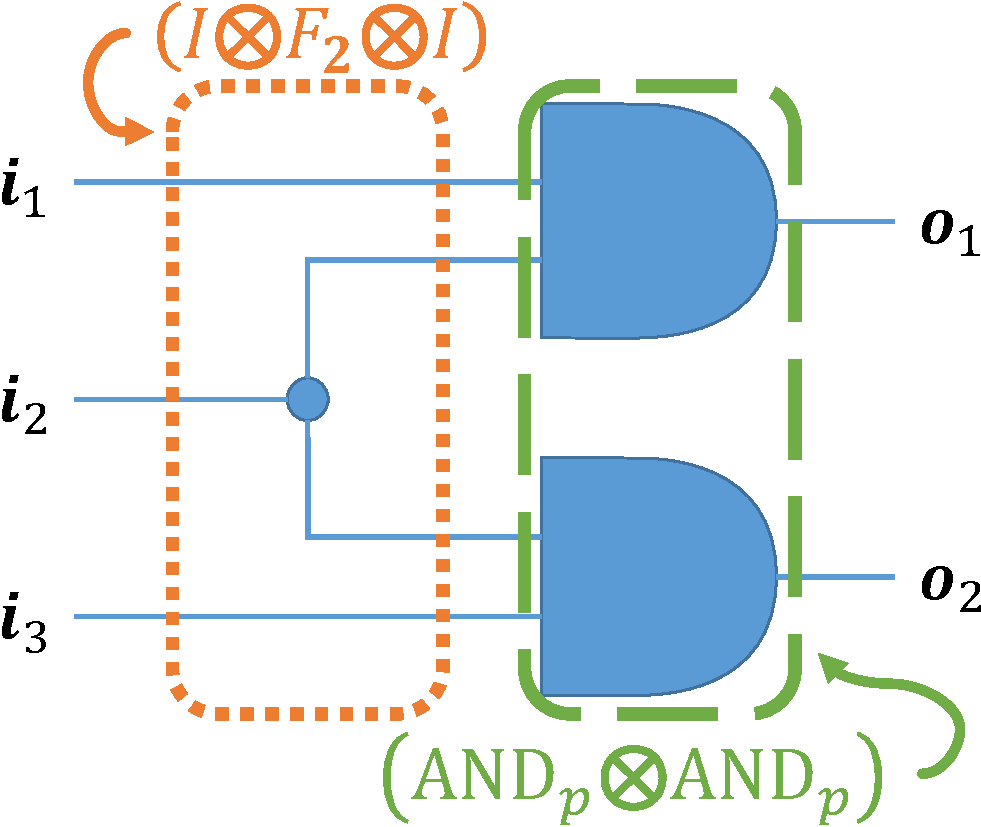
\includegraphics[height=60mm,clip]{img/exgate.pdf}
    \caption{組み合わせ回路の例}
    \label{fig:exgate}
  \end{center}
\end{figure}
また,図~\ref{fig:exgate} の回路に存在するような 2 個に分岐する部分は以下のように表す.
\[
F_2 = \left[
    \begin{array}{cccc}
      1 & 0 & 0 & 0\\
      0 & 0 & 0 & 1
    \end{array}
  \right]
\]


ゲートの直列接続に対応する PTM は,対応する PTM 同士の積に対応する.
一方,並行したゲートに対応する PTM は,対応する PTM 同士のテンソル積(クロネッカー積,$\otimes$)に対応する.
これらの計算を組み合わせることで,目的とする回路の PTM を得ることができる.

例えば,確率 $0.05$ で反転する AND ゲートを用いて図~\ref{fig:exgate} の回路を構成した時,
この回路に対応する PTM は式~(\ref{eq:ex-ptm}) のように求められる.
\begin{eqnarray}
  M_p &=& (I \otimes F_2 \otimes I)({\it AND}_p \otimes {\it AND}_p) \label{eq:ex-ptm} \\
    &=& \left(
    \left[
    \begin{array}{cccc}
      1 & 0\\
      0 & 1\\
    \end{array}
    \right]
    \otimes
    \left[
    \begin{array}{cccc}
      1 & 0 & 0 & 0\\
      0 & 0 & 0 & 1
    \end{array}
    \right]
    \otimes
    \left[
    \begin{array}{cccc}
      1 & 0\\
      0 & 1\\
    \end{array}
    \right]
    \right)
    \left(
    \left[
    \begin{array}{cc}
      0.95 & 0.05\\
      0.95 & 0.05\\
      0.95 & 0.05\\
      0.05 & 0.95
    \end{array}
    \right]
    \otimes
    \left[
    \begin{array}{cc}
      0.95 & 0.05\\
      0.95 & 0.05\\
      0.95 & 0.05\\
      0.05 & 0.95
    \end{array}
    \right]
    \right) \nonumber \\
  &=& \left[\begin{array}{cccc}
    0.9025 & 0.0475 & 0.0475 & 0.0025\\
    0.9025 & 0.0475 & 0.0475 & 0.0025\\
    0.9025 & 0.0475 & 0.0475 & 0.0025\\
    0.0475 & 0.9025 & 0.0025 & 0.0475\\
    0.9025 & 0.0475 & 0.0475 & 0.0025\\
    0.9025 & 0.0475 & 0.0475 & 0.0025\\
    0.0475 & 0.0025 & 0.9025 & 0.0475\\
    0.0025 & 0.0475 & 0.0475 & 0.9025
  \end{array} \right] \nonumber
\end{eqnarray}
最終的に得られた 8 行 4 列の行列から,各入力に対する出力の発生確率がわかる.
\redout{例えば,} $M_p(4, 2) = 0.9025$ からは,
$\bm i = 4 - 1 = (011)_2$: $i_1 = 0, i_2 = 1, i_3 = 1$ を入力した時,
0.9025 の確率で $\bm o = 2 - 1 = (01)_2$: $o_1 = 0, o_2 = 1$ が出力されることがわかる.

回路に故障が発生しない理想的な状況に対して PTM を計算すると,確率 $p$ は 0 もしくは 1 となる.
このような PTM を,特に Ideal Transfer Matrix (ITM) と呼ぶ.
図~\ref{fig:exgate} の回路に対応する ITM は,式~(\ref{eq:ex-itm}) のようになる.
\begin{eqnarray}
  M &=& (I \otimes F \otimes I)({\it AND} \otimes {\it AND}) \label{eq:ex-itm}\\
    &=& \left(
    \left[
    \begin{array}{cccc}
      1 & 0\\
      0 & 1\\
    \end{array}
    \right]
    \otimes
    \left[
    \begin{array}{cccc}
      1 & 0 & 0 & 0\\
      0 & 0 & 0 & 1
    \end{array}
    \right]
    \otimes
    \left[
    \begin{array}{cccc}
      1 & 0\\
      0 & 1\\
    \end{array}
    \right]
    \right)
    \left(
    \left[
    \begin{array}{cccc}
      1 & 0\\
      1 & 0\\
      1 & 0\\
      0 & 1\\
    \end{array}
    \right]
    \otimes
    \left[
    \begin{array}{cccc}
      1 & 0\\
      1 & 0\\
      1 & 0\\
      0 & 1\\
    \end{array}
    \right]
    \right) \nonumber \\
    &=& \left[
    \begin{array}{cccc}
      1 & 0 & 0 & 0\\
      1 & 0 & 0 & 0\\
      1 & 0 & 0 & 0\\
      0 & 1 & 0 & 0\\
      1 & 0 & 0 & 0\\
      1 & 0 & 0 & 0\\
      0 & 0 & 1 & 0\\
      0 & 0 & 0 & 1
    \end{array}
    \right] \nonumber
\end{eqnarray}

回路の最終的な信頼性は,式~(\ref{eq:fidelity}) のように,
正しい出力が得られる確率を,入力パターンが与えられる確率によって重み付き平均をとることによって評価する.
入力パターンが与えられる確率はベクトル ${\bm v}$ で表現し,${\bm i} + 1$ 番目の要素は,
${\bm i}$ を2進数としたときの入力パターンが与えられる確率を表している.
\begin{eqnarray}
  {\it fidelity}({\bm v}, M, M_p) = | {\bm v} (M_p .* M) |_{1} \label{eq:fidelity}
\end{eqnarray}
ここで, `$.*$' は要素ごとの乗算を表し, $| {\bm v} |_{1}$ は,ベクトル ${\bm v}$ の $l_1$-ノルム を表す.

%\todo[inline]{計算過程を全部書く}
図~\ref{fig:exgate} の回路に,全ての入力パターンが等確率で与えられる場合,
${\bm v}$ は,各要素は 0.125 で要素数 8 のベクトルとなる.
ここまでの例で計算した $M_p, M$ を用いて式~(\ref{eq:fidelity}) を計算すると,0.9025 という値が得られる.
\[
  M_p .* M = \left[\begin{array}{cccc}
      0.9025 & 0 & 0 & 0 \\
      0.9025 & 0 & 0 & 0 \\
      0.9025 & 0 & 0 & 0 \\
      0 & 0.9025 & 0 & 0 \\
      0.9025 & 0 & 0 & 0 \\
      0.9025 & 0 & 0 & 0 \\
      0 & 0 & 0.9025 & 0 \\
      0 & 0 & 0 & 0.9025
    \end{array}
  \right]
\]
\begin{eqnarray}
  {\it fidelity}({\bm v}, M, M_p) &=& \left|
  \left[
    \begin{array}{ccc}
      0.125 & ... & 0.125
    \end{array}
  \right] ( M_p .* M )
  \right|_{1} \nonumber \\
  &=& \left| \left[ \begin{array}{cccc}
    0.5640625 & 0.1128125 & 0.1128125 & 0.1128125
  \end{array} \right] \right|_{1} \nonumber \\
  &=& 0.9025 \nonumber
\end{eqnarray}
この結果は,ソフトエラーによって 0.05 の確率で反転する AND ゲートを用いて図~\ref{fig:exgate} の回路を構成した時,
全ての入力パターンが等確率で与えられることを仮定すると, 0.9025 の確率で正常に動作することを意味している.


\section{Algebraic Decision Diagram (ADD)を用いた計算}

% 導入
\ref{sec:ptm-const} 節の手法において,
計算の途中で発生する PTM のサイズは,指数的に大きくなる可能性がある.
与えられた 2 個の行列 $M_{1}, M_{2}$ のサイズが $k \times l$ と $m \times n$ のとき,
$M_{1} \otimes M_{2}$ のサイズは $km \times ln$ となる.
そのため,回路の中で並行した部分の入力と出力の数を $n', m'$ とすると,
$2^{n'} \times 2^{m'}$ のサイズの PTM が生成される.
この課題に対して, Algebraic Decision Diagram (ADD)
\cite{580054} を用いた手法 \cite{Krishnaswamy:2008:PTM:1297666.1297674} が提案された.
ADD は Binary Decision Diagram (BDD)~\cite{BLTJ:BLTJ1585} から派生したデータ構造で,
行列内の部分的に共通した情報を省略して保持しながら計算することができる.

% ADD の説明
ADD は,無閉路有向グラフ $(\Phi \cup V \cup T, E)$ として
$\{0, 1\}^n \mapsto S$ の関数の集合を表す.
\redout{ここで,}$S$ は定数の集合である.
$\Phi$ は入次数 0,出次数 1 の開始節点であり,その ADD で表現したい関数と 1 対 1 で対応する.
中間節点 $V$ は,関数が依存する変数を表して\redout{いるため},出次数は 2 となる.
この 2 個の辺は,1-枝と0-枝と呼ばれ\redout{る.
関数をの結果を得る際には,節点の変数に 0 を割り当てた場合は0-枝,
1 を割り当てた場合は1-枝をたどり,終端節点 $T$ を探索する.}
終端節点は,変数割り当ての結果として $S$ に含まれる定数でラベル付けされている.
BDD では論理関数を再帰的に表現し,終端節点は定数関数を表す 1 か 0 となる\redout{.
一方,}ADD では,終端節点の扱い方を変更し,0, 1 に限らない任意の終端節点を持つことができる.

\begin{figure}[tb]
  \centering
  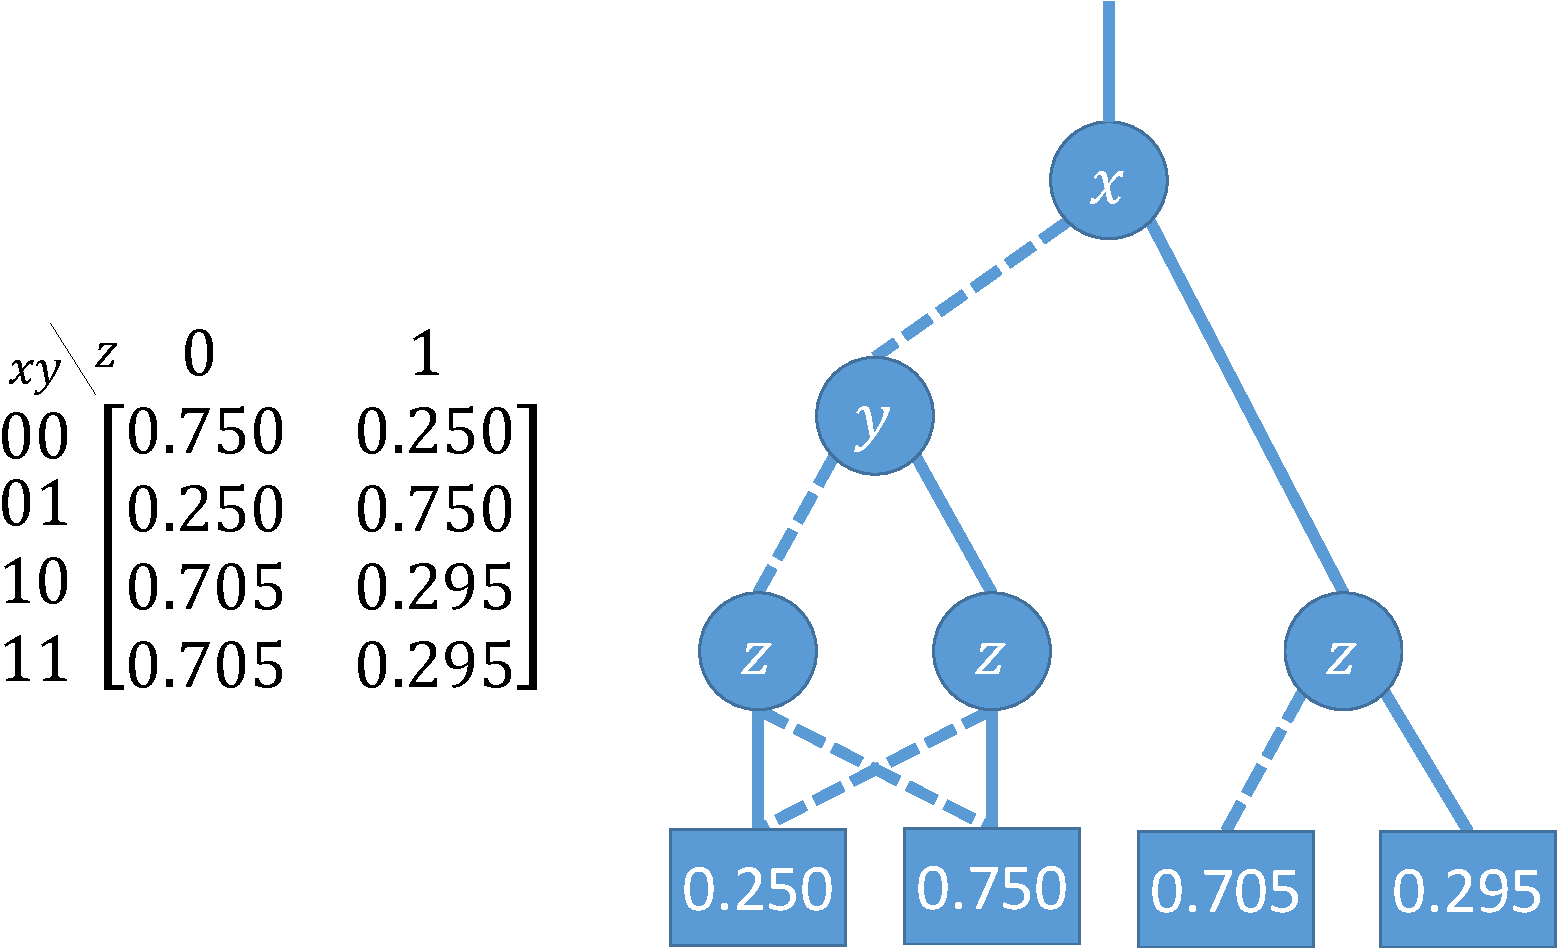
\includegraphics[height=70mm]{img/add-sample}
%  \missingfigure[figwidth=60mm]{ADD の画像を入れる}
  \caption{ADD によって行列を表現する例}
  \label{fig:ex-add}
\end{figure}
行列を ADD で表現した際のグラフ構造の例を図~\ref{fig:ex-add}に示す.
1-枝と0-枝は,それぞれ実線\redout{の}矢印と破線\redout{の}矢印で表されている.
各節点で場合分けを行う決定変数が 1 の場合は1-枝,0の場合は0-枝に対応し,
根節点から終端節点への 1 本のパスは, $\{0, 1\}^n$ と定数の対応を表している.
すなわち,各非終端節点は決定変数でラベル付けされて\redout{いるため},
決定変数の割り当て通りに\redout{枝を}たどることで,対応する定数を得ることができる.

\begin{figure*}[tb]
  \begin{minipage}{0.5\hsize}
    \centering
    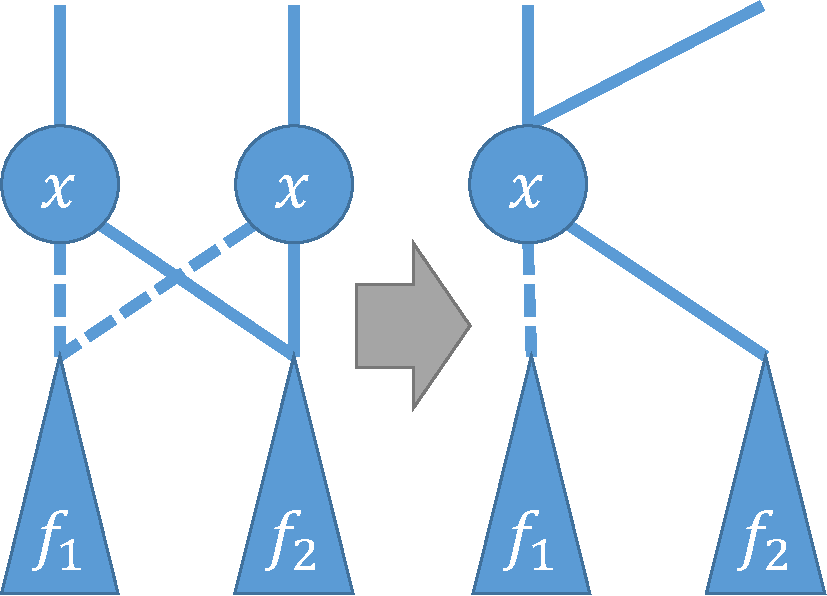
\includegraphics[height=50mm]{img/add-share-rule.pdf}
%    \missingfigure[figwidth=60mm]{サブグラフのマージ}
    \caption{等価な節点の共有}
    \label{fig:add-marge}
  \end{minipage}
  \begin{minipage}{0.5\hsize}
    \centering
    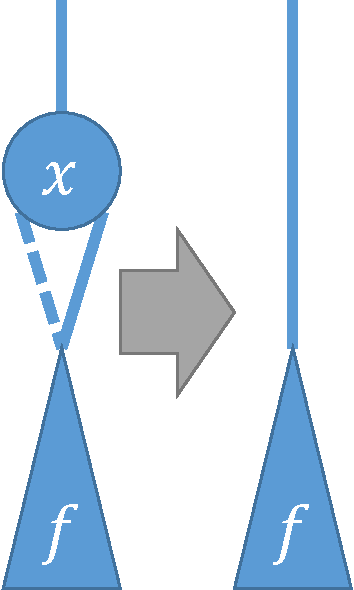
\includegraphics[height=50mm]{img/add-needlessly-rule.pdf}
%    \missingfigure[figwidth=60mm]{冗長な節点の削除}
    \caption{冗長な節点の削除}
    \label{fig:add-remove}
  \end{minipage}
\end{figure*}
ADD は変数の順序を固定し,等価な節点の共有と冗長な節点を削除することによって,
コンパクトかつ一意な表現を得ることができる.
2つの節点 $v_i, v_j$ が以下を満すとき,この2つの節点は等価であり,
図~\ref{fig:add-marge} のように共有することができる.
\begin{itemize}
  \item $v_i$ と $v_j$ \redout{にラベル付けされた決定変数が同じ}
  \item $v_i$ と $v_j$ の0-枝が同じ節点を指す
  \item $v_i$ と $v_j$ の1-枝が同じ節点を指す
\end{itemize}
$v_i, v_j$ が終端節点の場合には,ラベル付けされた定数のみを比較して等価性を判断する.
また,ある節点の0-枝と1-枝が同じ節点を指すとき,この節点は冗長なので,
図~\ref{fig:add-remove} のように削除することができる.
図中の $f_1, f_2, f$ は ADD の部分グラフである.

また,2 個の ADD を入力し,それらの二項演算の結果を直接生成するアルゴリズムが考案されている.
これらのアルゴリズムは,
一意性についてのキャッシュテーブルと演算についてのキャッシュテーブルを利用することで効率的に計算することができる.
ADD を用いて PTM を計算する手法では,必要な演算を追加で定義し,同様の効率性を持ったまま計算することができる.

%\chapter{Zero-suppressed Binary Decision Diagram}
%\todo[inline]{TODO: ZDD の数式処理がうまくいったら入れる}

\chapter{信頼性の効率的計算手法}\label{sec:proposed}
%\todo[inline]{TODO: 2章の文字の定義,ノード/節点/頂点,辺/弧を合わせる}

ADD \redout{を用いると},等価な節点の共有や冗長な節点の削除によって,
行列内の部分的に共通した情報を省略して表現できる.
\cyannout{しかし,行列はテンソル積によって急激に増加するため,
ADD による圧縮では不十分であると考えられる.
ADD の終端節点は,行列に含まれる値の種類数だけ存在するため,
行列のサイズが増加すれば,終端節点の数も増加しやすくなるからである.
終端\greenout{節}点の数が増加すると,それらを区別するための節点も増加し,
ADD のサイズは行列のサイズと相関する可能性がある.}

\cyannout{また,各ゲートに与えられる $p$ の値は,全て同じ値とは限らない.
既存手法では,全てのゲートで $p = 0.05$ 用いて\blueout{実験を行った}ため,
同じ部分行列が発生しやすく,ADD に適した状況となっている.
逆に,ゲートの出力が反転する確率として,いくつかの異なる値を設定した場合は,
節点の共有が発生しづらく,ADD \greenout{では対処できない}状況となることが予想される.}
\cyannout{大規模で多様な回路を評価するためには,}より効率的な計算方法が必要と\redout{考えられる}.

\section{評価式の変形による効率化手法}\label{sec:prop:deform}

%\paragraph{(${\it fidelity}({\bm v}, M, M_p) = {\bm v} \cdot {\bm s}$ について)}
既存手法では,行列 $M_p, M$ のサイズが問題となる.
そこで,提案手法ではこの行列を用いずに, $M_p .* M$ と等価な値を得る別のアプローチを検討する.

$M_p .* M$ は,正しい出力以外を 0 にする計算とみなすことができる.
$M_p .* M$ から,行ごとに 0 以外の要素を抜き出したベクトル ${\bm s}$ を用いると,
式~(\ref{eq:fidelity}) の値は,内積を用いて以下のように求めることができる.
\begin{eqnarray}
  {\it fidelity}({\bm v}, M, M_p) = {\bm v} \cdot {\bm s} \label{eq:deformed}
\end{eqnarray}

$M_p .* M$ が正しい出力を抜き出す処理と考えると, ${\bm s}$ の $\bm{i} + 1$ 番目の要素は,
2 進数として表したビット列 ${\bm i}$ を入力したときに正しい出力が得られる確率である.
\ref{sec:ptm-const} 節の例と同じ状況
(図~\ref{fig:exgate} の回路を,0.05 の確率で反転するゲートを用いて構成し,入力パターンが等確率で与えられる場合)
ならば, ${\bm s}$ は各要素が 0.9025 で要素数 8 のベクトルとなり,
行列を計算することなく, ${\bm v} \cdot {\bm s} = 0.9025$ が得られる.

\subsection{正しい出力が得られる確率の計算}

% 文字の定義
${\bm s}$ の各要素は,
組み合わせ回路 $C$ を無閉路有効グラフ $G_C = ({\it PI} \cup {\it PO} \cup V_C, E_C)$ として表し,
再帰的に計算することで求められる.
% 頂点について
${\it PI}, {\it PO}$ は,それぞれ外部入力と外部出力を表す頂点集合であり,
$V_C$ は,各ゲートの頂点集合である.
ゲート $g \in V_C$ が確率 $p$ で反転するとき, $err(g) = p$ とする.
% 辺について
ある頂点 $g'$ の出力が,頂点 $g$ に入力されている時,
2 個の頂点は入力される側から出力する側への有向辺 $(g, g') \in E_C$ で結ばれる.
また,頂点 $g$ のファンインを ${\it FI}(g)$,ファンアウトを ${\it FO}(g)$ で表す.
$g$ の入次数は $|{\it FI}(g)|$,出次数は $|{\it FO}(g)|$ となる.
$g \in {\it PI}$ の場合には $|{\it FI}(g)| = 0$ であり,
$g \in {\it PO}$ の場合には $|{\it FO}(g)| = 0$ である.

%\paragraph{(${\bm s}$ を計算するアルゴリズムについて)}
全ての外部出力が正しく出力されれば,正しい出力が得られている.
回路に ${\bm i}$ を入力した時のゲート $g$ が誤りとなる確率 ${\it fail}({\bm i}, g)$ とすると,
${\bm s}$ の各要素は以下のようになる.
\begin{eqnarray}
  {\bm s}({\bm i} + 1) = \prod_{g \in PO}(1 - {\it fail}({\bm i}, g)) \label{eq:allnofail}
\end{eqnarray}

${\bm i}$ を入力した時にゲート $g$ が誤りとなる確率 ${\it fail}({\bm i}, g)$ は,
ゲートのファンインで考えられる全てのエラーパターンに分けて考える.
エラーのパターンはビット列 ${\bm e}$ を用いて表す.
例えば, $|{\it FI}(g)| = 3$ のゲートに $(011)_2$ を入力し,
${\bm e} = (010)_2$ のエラーが発生した時,
ビット同士の XOR によって $(010)_2$ が入力されると考える.
全てのエラーパターン集合は,$\{0, 1\}^{|{\it FI}(g)|}$ で得ることができる.
\cyannout{すなわち,}頂点 $g$ でエラーパターン ${\bm e}$ が発生し,
\blueout{同時に反転の状態を出力が誤りとなるような}確率を求める.
\begin{eqnarray}
  {\it fail}({\bm i}, g) = {\displaystyle \sum_{{\bm e} \in \{0, 1\}^{|{\it FI}(g)|}}}
    O({\bm i}, g, {\bm e}) \times {\it toFail}({\bm i}, g, {\bm e}) \label{eq:fail}
\end{eqnarray}
ただし,$g \in {\it PI}$ の時,反転が発生することはないので,
\begin{eqnarray}
  {\it fail}({\bm i}, g) = 0
\end{eqnarray}
とする.

エラーパターン ${\bm e}$ の生起確率は,前段の頂点 $g'$ から計算される.
\begin{eqnarray}
  O({\bm i}, g, {\bm e}) = \prod_{\substack{g' \in {\it FI}(g),\\ e_{g'} \in {\bm e}}} \begin{cases}
    {\it fail}({\bm i}, g') & : e_{g'} = 1\\
    1 - {\it fail}({\bm i}, g') & : e_{g'} = 0
  \end{cases} \label{eq:occur}
\end{eqnarray}
${\bm e}$ の $i$ 番目の要素が 1 の時,$g$ の $i$ 番目の出力が誤って入力される確率が与えられる.
すなわち,式~(\ref{eq:occur}) は,全てのファンインが同時に ${\bm e}$ の表す状態になる確率を求めている.

${\it toFail}({\bm i}, g, {\bm e})$ は,ゲート $g$ が最終的に誤った出力となるように反転する確率である.
回路に ${\bm i}$ を入力した時のゲート $g$ の正しい出力を ${\it out}({\bm i}, g)$ とし,
${\bm i}$ を入力してエラーパターン ${\bm e}$ が発生した時のゲート $g$ の出力を
${\it act}({\bm i}, g, {\bm e})$ とする.
%これらの結果を比較して,このゲートが反転するべきかどうかを判断し,\blueout{式~(\ref{eq:to_fail})} のように計算する.
これらの結果から,\blueout{このゲートが誤った出力となるためには,}反転\blueout{した状態になる}べきかどうかを判断し,\blueout{式~(\ref{eq:to_fail})} のように計算する.
\begin{eqnarray}
  {\it toFail}({\bm i}, g, {\bm e}) = \begin{cases}
    {\it err}(g) & : {\it out}({\bm i}, g) = {\it act}({\bm i}, g, {\bm e})\\
    1 - {\it err}(g) & : {\it out}({\bm i}, g) \neq {\it act}({\bm i}, g, {\bm e})
  \end{cases} \label{eq:to_fail}
\end{eqnarray}
入力の誤りに関わらず,論理マスクの影響によって正しい出力が得られる場合,
ゲート $g$ は\blueout{出力が誤りになるように}反転しなくてはならない.
一方,入力の誤りが出力に影響を与え,最終的に誤った出力となる場合には,
ゲート $g$ はその誤った出力を次のゲートへ入力する必要がある.
例えば,\greenout{2 入力の AND ゲート $g$ が存在する回路の外部入力に \blueout{${\it bin}({\bm i})$} を与えた結果,
\cyannout{回路内に存在する} AND ゲート $g$ に $(00)_2$ が入力された}とする.
このとき,正しいゲートの出力は ${\it out}({\bm i}, g) = 0$ となる.
ゲート $g$ の出力が本来とは異なるようになるためには,
$bin({\bm e}) = (11)_2$ の場合に反転せず,それ以外では反転しなくてはな\blueout{ら}ない.

式~(\ref{eq:fail}) の $O({\bm i}, g, {\bm e}) \times {\it toFail}({\bm i}, g, {\bm e})$ は,
エラーパターン ${\bm e}$ が発生し,かつ,
そのエラーパターンの時に最終的なゲート $g$ の出力が正しい値から反転する確率を求めている.
全てのエラーパターンについて場合分けを行い,それぞれの状態についての確率の和\greenout{を求めることで},
そのゲートの出力が誤りとなる確率\greenout{を得る}.

%\paragraph{(擬似コードを用いた議論)}
\begin{algorithm}[tbp]
  \caption{{\bf fail}: 与えられたノードの出力が反転する確率を求める}
%  \caption{{\bf fail}: Calculating a probability that gate $g$ outputs an incorrect galue}
  \label{alg:failprob}
  \begin{algorithmic}[1]
    \REQUIRE ${\it g}$: 出力のエラー率を求めるノード
%    \REQUIRE ${\it g}$: the gate for the calculation
    \IF{$g \in PI$}
      \RETURN 0
    \ENDIF
    \IF{$g$ はすでに計算済み}
      \RETURN ${\it fail\_cache}[g]$
    \ENDIF
    \STATE ${\it res} = 0$
    \FORALL{${\bm e} \in \{0, 1\}^{|{\it FI}(g)|}$}
      \STATE $O \leftarrow 1$
      \FORALL{$g' \in {\it FI}(g), e_{g'} \in {\bm e}$}
        \IF{$e_{g'} = 1$}
          \STATE $O \leftarrow O \times {\it fail}(g')$
        \ELSE
          \STATE $O \leftarrow O \times (1 - {\it fail}(g'))$
        \ENDIF
      \ENDFOR
      \STATE ${\it res} \leftarrow {\it res} + O \times {\it toFail}(g, {\bm e})$
    \ENDFOR
    \STATE ${\it fail\_cache}[g] \leftarrow res$
    \RETURN ${\it res}$
  \end{algorithmic}
\end{algorithm}
実際の計算では,各入力を終端ノードに設定してから Algorithm~\ref{alg:failprob} のように再帰的に計算を行う.
9-16行目が式~\ref{eq:occur} の計算に相当する.
${\it toFail}$ の計算に用いる ${\it out}$ の値は,入力の設定時に事前に計算することができる.
また,${\it act}$ の値は, ${\it out}$ と ${\bm e}$ を用いて計算できる.
この計算は,全ての出力線から開始しなくてはならない.

関数 ${\it fail}$ の結果は,入力パターンとノードの組に対して一意に定まるので,
一度求めた結果は再利用することができる.
具体的には,Algorithm~\ref{alg:failprob} に加えて, $g$ に対する値を計算していないか調べ,
存在すればその値を返すような処理行なえばよい.
また,入力パターンを変更するごとに計算結果を\cyannout{消去}している.
したがって,1 個の入力パターンに対しては,
\greenout{式~(\ref{eq:allnofail})} のように $|PO|$ 回だけ再帰を開始しなくてはならないが,
パターンを設定してから\greenout{ 2 個}目以降の外部出力に対する結果は,
過去に計算した値を利用できる場合があるため比較的少ない時間で求められると期待できる.

%\paragraph{(ゲートの分割)}
Algorithm~\ref{alg:failprob} の 8-18 行目のループは,
一度の呼び出しで $2^{|FI(g)|} \times |FI(g)|$ 回実行される可能性がある.
そこで,4 入力以上を持つゲート ($|FI(g)| \geq 4$) は,2 入力のゲートに分割して計算しなくてはならない.
このとき,元のゲートの出力が反転する確率と,分割後の最終段のゲートの出力が反転する確率は等しく,
それ以外は反転を発生しないゲートとする.
このように回路を変形させることで,$2^{|FI(g)|} \times |FI(g)|$ 回のループを,
$2^3$ 回のループを含んだ $|FI(g)| - 1$ 回の関数呼び出しに置き換えることができる.

\subsection{異なる入力間での計算結果の再利用}\label{sec:prop:deform:reuse}

%The calculation can also start from the nodes corresponding the primary inputs
%by the topological order instead of the above method.
関数 ${\it fail}$ は,外部入力側のノードからトポロジカル順に計算することもできる.
%It is enough to calculate the output of a gate whose input values are changed
%since the probability of flipping depends on the input values.
このとき,最終的に出力が誤る確率は入力に依存するため,
変化した入力に依存したノードのみを更新すれば十分である.
\begin{figure}[tbp]
  \begin{center}
    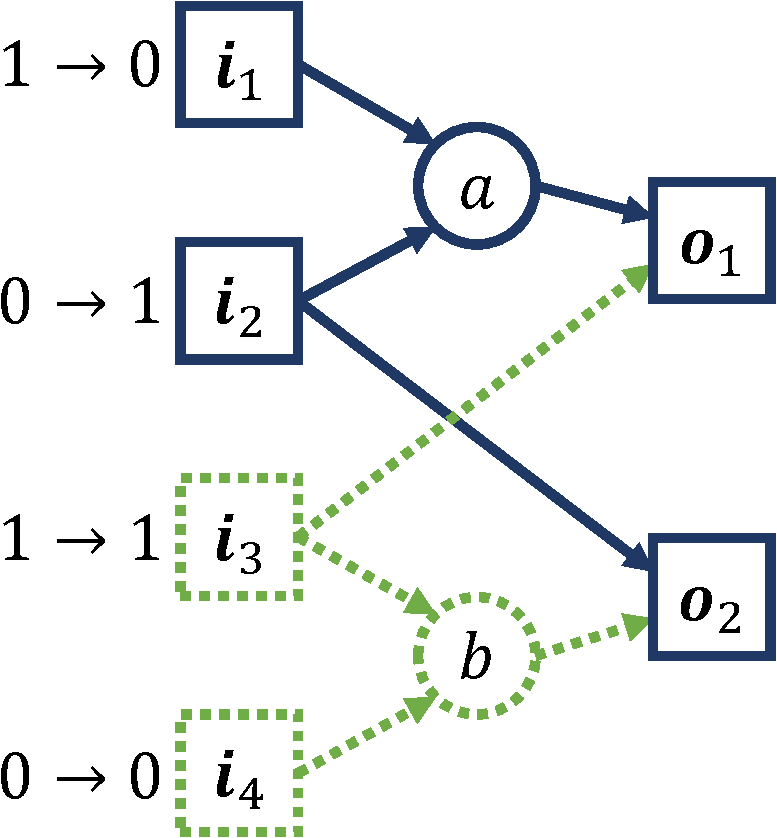
\includegraphics[width=64mm,clip]{img/update_graph.pdf}
  \end{center}
%\caption{4入力2出力の回路の例と再計算}
%  \caption{Recalculation when the input pattern is changed
%  where a circuit which has four primary inputs, two primary outputs and two gates}
  \caption{4入力2出力の回路ににおける入力パターンが変更した際の再計算}
\label{fig:update_graph}
\end{figure}
%Fig.~\ref{fig:update_graph} shows the recomputation in the nodes depending on the changed inputs.
図~\ref{fig:update_graph} は入力が変化した際に,再計算を行うノードを示している.
%In this example, the calculation starts from nodes ${\bm i}_1$ and ${\bm i}_2$
%and updates node $a$, ${\bm o}_1$ and ${\bm o}_2$ in order.
この例では,入力が変化した ${\bm i}_1, {\bm i}_2$ から開始して,$a, {\bm o}_1, {\bm o}_2$ の順に更新する.
%We do not have to calculate the probability on node $b$
%since the dependent nodes: both ${\bm i}_3$ and ${\bm i}_4$, do not change their values.
${\bm i}_3, {\bm i}_4$ の入力は変化しないため,これらのみに依存するノード $b$ は更新する必要がない.
このようにすると,変化した入力に依存するノードのみを再計算できる.

%\paragraph{(グレイコードを用いる)}
計算順序の変更に加えて,入力パターンの割り当てにグレイコードを用いることで,
さらに計算時間を短縮できる.
%In addition to the reverse of the calculation order, assignment of the input pattern by Gray Code saves time.
%Gray Code can enumerate all the input patterns such that the two adjacent input patterns differs at only one bit.
%Then we can reduce the started nodes to recalculate.
グレイコードは,1ビットのみを変更させながら,全ての入力パターンを列挙できるため,
再計算が開始されるノードを減らすことができるからである.
%When we generate the input patterns by the simple ascending order of binary number,
%there is a case that multiple inputs are changed between two input patterns.
入力パターンを単純な2進数を用いて0から順番に割り当てると,
全てのビットが変化してしまうケースが存在する.
%e.g. $(011)_2 \to (100)_2$ (We need start from the three nodes since the assignment of the three inputs are different).
例えば,$(011)_2 \to (100)_2$ のような変化は,3 箇所のが変化し,3 個のノードから開始しなくてはならない.
%Therefore, by using Gray Code, we can start from the single node at all times after the calculation of the first pattern.
それに対し,グレイコードを用いると,
2つ目以降の入力パターンについては,常に 1 個のノードから再計算をするだけで十分となる.

\subsection{正しい確率が得られないケース}

\begin{figure}[tbp]
  \begin{center}
    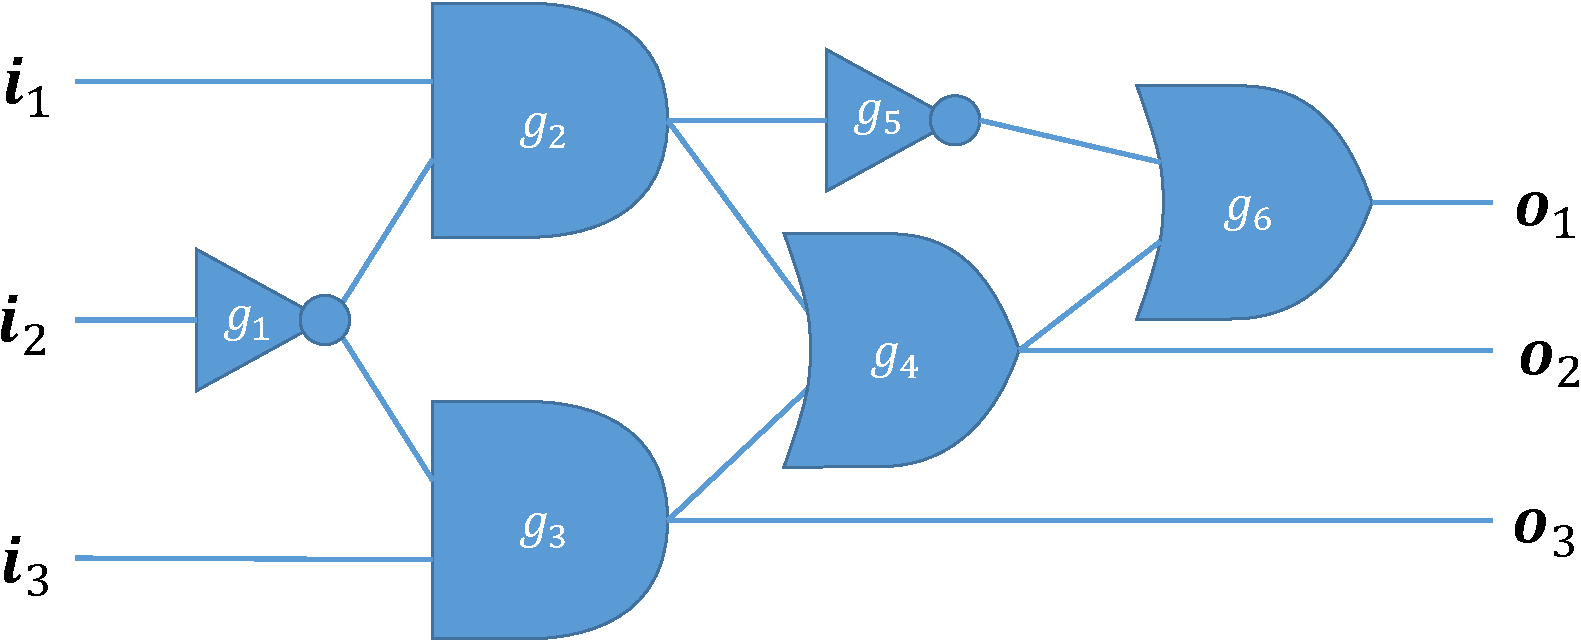
\includegraphics[height=50mm,clip]{img/join.pdf}
  \end{center}
  \caption{2 箇所の再収斂によって正確な結果が得られない例}
  \label{fig:join}
\end{figure}
%Our method may calculate inaccurate probabilities
%if the circuit contains fan-out points which may reconverge later.
ここまで提案してきた手法では,回路に再\greenout{収}斂を含むケースに対して正確な結果を得ることができない.
%When we use the method just as it is, the result contains a contradicted suppositions
%that the different soft-error occurrence at the same gate between inputs.
回路に再\greenout{収}斂が含まれている場合,計算結果には,
同一のゲートに対して異なるソフトエラー発生の状態を仮定した計算が含まれてしまうからである.
%TODO グラフの分割と合成
%In the case of Fig~\ref{fig:join}, the inputs of gate $g_4$ branch from the outputs of gate $g_1$.
例えば,図~\ref{fig:join} のようなケースにおいて,$g_1$ から分岐した出力は $g_4$ へ 2 通りの経路から入力される.
%Then the calculation at gate $g_2$ suppose that the error occur or does not occur,
%この時,ゲート $g_4$ の結果は,ゲート $g_1$ でエラーが起きた場合と起きない場合の両方の仮定を用いている.
この時,ゲート $g_4$ の結果は,\redout{ゲート $g_1$ でエラーが起きた場合と起きない場合の矛盾した仮定を用いているため,
ここまで述べてきた手法では,誤った値を計算していることになる}.
%and the calculation at gate $g_3$ also supposes that.
また,ゲート $g_3$ の結果も両方の仮定を用いている.
%In the calculation at gate $g_4$, even though the calculation of $g_2$ supposes that the error occur,
したがって,$g_4$ での計算は,$g_2$ の計算で $g_1$ にエラーが発生しないと仮定したにもかかわらず,
%the calculation of $g_4$ contains the cases supposing that the error does not occur.
$g_4$ の計算で $g_1$ にエラーが発生すると仮定して計算した場合を含んでしまう.
%The calculation at gate $g_5$ also contains supposition.
ゲート $g_2$ の分岐でも,同様に\redout{矛盾した仮定を用いて計算してしまう}.
%However, it should be noted that this kind of errors would not be so problematic
%in many cases as our experimental results show in the next section.
%しかしながら,少なくとも本研究で行った実験ではこのようなケースはそれほど大きな誤差を引き起こさない.

\section{数式処理による計算手法}\label{sec:prop:exp}

% 概要

関数 ${\it fail}$ の計算において誤った結果となってしまうのは,
同一のゲートについて,実際には発生しない状態を仮定をしてしまうからである.
そこで,再\greenout{収}斂の元となるファンアウト・ポイントに対し変数を定義することで,
この状態の計算を修正することを考える.

\subsection{補正ルールの検討}

\begin{figure}[tbp]
  \begin{center}
    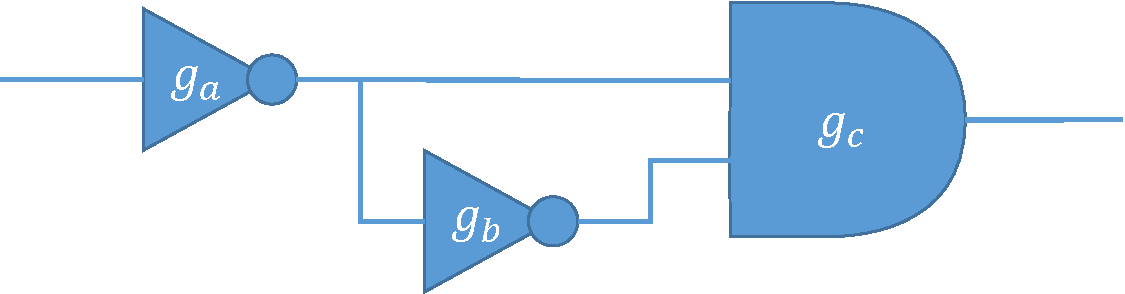
\includegraphics[height=25mm,clip]{img/min-reconv.pdf}
  \end{center}
  \caption{再収斂が 1 箇所存在するケース}
  \label{fig:min-reconv}
\end{figure}
再収斂が問題となるケースとして,図~\ref{fig:min-reconv} のような回路を考える.
ここで,ゲート $g_a$ の出力が異なる状態を仮定してしまうのが問題である.
そこで,ゲート $g_a$ の出力が最終的に 1 となる確率を $P(g_a)$ とおく.
他のゲートについて出力が 1 となる確率を求めると,以下のようになる.
\begin{eqnarray}
P(g_b) &=& P(g_a) {\it err}(g_b) + (1 - P(g_a)) (1 - {\it err}(g_b)) \nonumber \\
P(g_c) &=& P(g_a \cap g_b) (1 - {\it err}(g_c)) + (1 - P(g_a \cap g_b)) {\it err}(g_c) \nonumber
\end{eqnarray}
$g_b$ は $g_a$ に依存して\redout{いるため},
\redout{ゲート $g_a, g_b$ の出力}が同時に 1 になる確率は,$P(g_a) P(g_b)$ では正しく計算出来ない.
\[ P(g_a) P(g_b) = P(g_a)^2 {\it err}(g_b) + P(g_a) (1 - P(g_a)) (1 - {\it err}(g_b)) \]
\redout{ゲート $g_a, g_b$ の出力}が同時に 1 になる正しい確率は,
\[ P(g_a \cap g_b) = P(g_a) {\it err}(g_b) \]
である.
そこで,3 種類の状況について,以下のように補正する.
\begin{description}
  \item[補正ルール 1] $P(g_i)^2 \rightarrow P(g_i)$
  \item[補正ルール 2] $(1 - P(g_i))^2 \rightarrow (1 - P(g_i))$
  \item[補正ルール 3] $P(g_i) (1 - P(g_i)) \rightarrow 0$
\end{description}
{\bf 補正ルール 2} は,出力が 0 となる場合について {\bf 補正ルール 1} と同様に補正することを示している.
また,同一のゲートであるため,反転が発生する状態と発生しない状態は同時に起こり得ない.
そこで {\bf 補正ルール 3} のように 0 に置き換える.

ここで,\redout{{\bf 補正ルール2},{\bf 補正ルール3} の左辺を展開し,
{\bf 補正ルール1} を}適用した場合,
\begin{description}
  \item[補正ルール 2] $(1 - P(g_i))^2 = 1 - 2 P(g_i) + P(g_i)^2 \rightarrow (1 - P(g_i))$
  \item[補正ルール 3] $P(g_i) (1 - P(g_i)) = P(g_i) - P(g_i)^2 \rightarrow 0$
\end{description}
となるため,{\bf 補正ルール1} のみを適用するだけで十分であるということがわかる.

\subsection{補正ルールを考慮した数式処理システム}

\redout{{\bf 補正ルール1} を適用するため}には,計算途中の情報を数式として保持する方法が考えられる.
再\greenout{収}斂されるノードでは,$P(g_i)$ を区別できないため,
\redout{単に数値として確率を表現している場合に}は,補正ルールを適用することができないからである.
そこで,補正ルールを考慮した数式処理システムを構築する.

$P(g_i)$ を記号として保持し,乗算の演算を行う際に補正ルールを適用させながら数式を処理する.
この時,$P(g_i)^2 \rightarrow P(g_i)$ のルールから,
2 以上の整数を $t$ として $P(g_i)^t \rightarrow P(g_i)$ が考えられる.
%したがって,現れる数式の項は 2 以上の指数を考える必要が無く,係数と変数の集合だけを管理すればよい.
\redout{したがって,現れる数式の各変数に関して 2 次以上の項}を考える必要が無く,係数と変数の集合だけを管理すればよい.

% 方針と項の表現方法
のちに再収斂が発生するファンアウト・ポイントの集合を $R$ で表す.
すなわち,$g \in R$ ならば,$P(g)$ は数式中で変数として表現しなくてはならない.
2 以上の指数を考えない場合,係数と変数の組み合わせの組で項を表し,
その集合によって以下のように数式を表現することができる.
\begin{eqnarray}
  F_e = \{ ({\it coeff}, {\it vars}) | {\it vars} \in \{0, 1\}^{|R|}, {\it coeff} = F({\it vars}) \}
\end{eqnarray}
例えば,$R = \{a, b\}$ において,$F(a, b) = 3ab + b$ を表す場合を考えると,
\[ F(0, 0) = F(1, 0) = 0 \]
\[ F(0, 1) = 1, F(1, 1) = 3 \]
\[ F_e = \{ (0, (0, 0)), (1, (0, 1)), (0, (1, 0)), (3, (1, 1)) \} \]
となる.
提案手法に必要な演算は,加減算と乗算である.
上記のように数式を表現した場合,これらの演算は集合の操作によって実現することができる.

\begin{algorithm}[tbp]
  \caption{{\bf operator} $+$: 数式同士の加算}
  \label{alg:add}
  \begin{algorithmic}[1]
    \REQUIRE $F_e, G_e$: 加算を行う多項式を表す集合
      \STATE ${\it result} \leftarrow \COMMENT{ハッシュテーブル} \varnothing$
      \FORALL{$({\it coeff}, {\it vars}) \in F_e \cup G_e$}
        \STATE ${\it result}[{\it vars}] \leftarrow ({\it result}[{\it vars}] {\mbox ~or~ } 0) + {\it coeff}$
      \ENDFOR
    \RETURN ${\it result}$
  \end{algorithmic}
\end{algorithm}
加算は,項の変数の組み合わせごとに分類し,係数の合計を求めれば良い.
加算のアルゴリズムを Algorithm~\ref{alg:add} に示す.
このアルゴリズムによって,${\it vars}$ と ${\it coeff}$ の対応が得られるので,
そこから $({\it coeff}, {\it vars})$ の集合を生成することができる.
同様のアルゴリズムを用いて,減算も実現することができる.

\begin{algorithm}[tbp]
  \caption{{\bf operator} $\times$: 数式同士の {\bf 補正ルール1} を適用した乗算}
  \label{alg:times}
  \begin{algorithmic}[1]
    \REQUIRE $F_e, G_e$: 乗算を行う多項式を表す集合
      \STATE ${\it result} \leftarrow \COMMENT{ハッシュテーブル} \varnothing$
      \FORALL{$(t_F, t_G) \in F_e \times G_e$}
        \STATE ${\it vars} \leftarrow (t_F.{\it vars} \; | \; t_G.{\it vars})$
        \STATE ${\it coeff} \leftarrow (t_F.{\it coeff} \; | \; t_G.{\it coeff})$
        \STATE ${\it result}[{\it vars}] \leftarrow ({\it result}[{\it vars}] {\mbox ~or~ } 0) + {\it coeff}$
      \ENDFOR
    \RETURN ${\it result}$
  \end{algorithmic}
\end{algorithm}
乗算は, 2 個の数式に含まれる項について乗算を行い,加算と同様に分類する.
乗算のアルゴリズムを Algorithm~\ref{alg:times} に示す.
ここで, `$|$' は要素同士の OR を表す.
項同士の乗算は,係数部分と変数部分に分けて行われ,
変数部分については,要素同士の OR で計算できる.

Algorithm~\ref{alg:add},~\ref{alg:times} で示された通り,
数式の演算にはハッシュテーブルが必要となる.
したがって,${\it vars}$ についてはハッシュ値を計算しなくてはならない.
${\it vars}$ がビット列で表されている場合には,ビット数に比例する時間でハッシュ値を計算できる.
あるいは,変数の組み合わせを,単一の組み合わせのみを含む特殊な
Zero-suppressed BDD (ZDD)~\cite{zdd-app} として表すこともできる.
同一の組み合わせかどうかは ZDD の節点番号を用いて判別でき,
ハッシュ値もこの節点番号を用いれば良い.
要素同士の OR は, ZDD の Join 演算~\cite{knuth2014art} を用いて実現できる.

%\todo[inline]{今後の課題に「係数を開始側に置くか終端側に置くか」を追加}

\subsection{数式の生成}

% アルゴリズムの書き換え

\begin{algorithm}[tbp]
  \caption{$P(g)$: 与えられたノードの出力が 1 になる確率についての数式を求める}
%  \caption{{\bf fail}: Calculating a probability that gate $g$ outputs an incorrect galue}
  \label{alg:oneex}
  \begin{algorithmic}[1]
    \REQUIRE ${\it g}$: 出力のエラー率を求めるノード
%    \REQUIRE ${\it g}$: the gate for the calculation
    \IF{$g \in PI$ もしくは,$g$ はファンアウト・ポイント}
      \RETURN\COMMENT{ 記号としての } $P(g)$
    \ENDIF
    \IF{$g$ はすでに計算済み}
      \RETURN ${\it one\_ex\_cache}[g]$
    \ENDIF
    \STATE ${\it res} = 0$
    \FORALL{${\bm b} \in \{0, 1\}^{|{\it FI}(g)|}$}
      \STATE $O \leftarrow 1$
      \FORALL{$g' \in {\it FI}(g), b_{g'} \in {\bm b}$}
        \IF{$b_{g'} = 1$}
          \STATE $O \leftarrow O \times P(g')$ \COMMENT{ ルールを適用した数式としての計算 }
        \ELSE
          \STATE $O \leftarrow O \times (1 - P(g'))$ \COMMENT{ ルールを適用した数式としての計算 }
        \ENDIF
      \ENDFOR
      \STATE ${\it res} \leftarrow {\it res} + O \times {\it toBeOne}(g, {\bm b})$ \COMMENT{ ルールを適用した数式としての計算 }
    \ENDFOR
    \STATE ${\it one\_ex\_cache}[g] \leftarrow res$
    \RETURN ${\it res}$
  \end{algorithmic}
\end{algorithm}
数式は,後に再収斂するファンアウト・ポイントで分割し,各部分回路ごとに生成する.
各ゲートの出力が 1 になる確率を計算する数式を生成するアルゴリズムは Algorithm~\ref{alg:oneex} のようになる.
${\it fail}$ の計算と同様,入力パターンの生起確\greenout{率}と,その入力の際に 1 になる確率によって計算できる.
${\it toBeOne}$ はゲートにビット列 ${\it bin}({\bm b})$ を入力した際に,ゲート\redout{の出力}が 1 になるための確率を返す.
この関数は式~(\ref{eq:to_be_one}) の様に計算できる.
\begin{eqnarray}
  {\it toBeOne}(g, {\bm b}) = \begin{cases}
    {\it err}(g) & : {\it logic}(g, {\bm b}) = 0 \\
    1 - {\it err}(g) & : {\it logic}(g, {\bm b}) = 1
  \end{cases} \label{eq:to_be_one}
\end{eqnarray}
このとき,${\it logic}(g, {\bm b})$ は,ゲート $g$ にビット列 ${\bm b}$ を入力した際の出力を返す.

\cyannout{ある入力について構成された数式は,他の入力においても再利用できる.
これは,入力を 0 から 1 に変えることと,外部入力が反転する確率が 0 から 1 になることが等価であるからである.
そこで,のちに再収斂が発生するファンアウト・ポイントの集合 $R$ に加え,
外部入力 ${\it PI}$ に含まれるノードについても変数として扱う.
したがって,$P(g), g \in \{ R \cup {\it PI} \}$ を変数とした数式が生成され,
各外部入力が 1 になる確率を与えることで,外部入力の信頼性を計算できる.}

${\bm s}$ の導出は,外部入力からトポロジカル順に,$P(g)$ へ値を割り当てることで求めることができる.
$P(g)$ は,1 となる確率であるから,$g_i \in PI$ の場合は,
1 を入力する場合は $P(g_i) = 1$,0 を入力する場合は $P(g_i) = 0$ とすればよい.
Algorithm~\ref{alg:oneex} によって,部分回路の出力が 1 となる確率を得ることができるので,
その結果を,対応するファンアウト・ポイントの変数へ代入することで,さらに別な部分回路の出力について計算できる.
全ての部分回路について計算すると,外部出力が 1 となる確率を得ることができ,
別に計算した ${\it out}({\bm i}, v)$ の結果と合わせて,
正しい出力が得られる確率 ${\bm s}({\bm i} + 1)$ を得る.

\begin{figure}[tbp]
  \begin{center}
    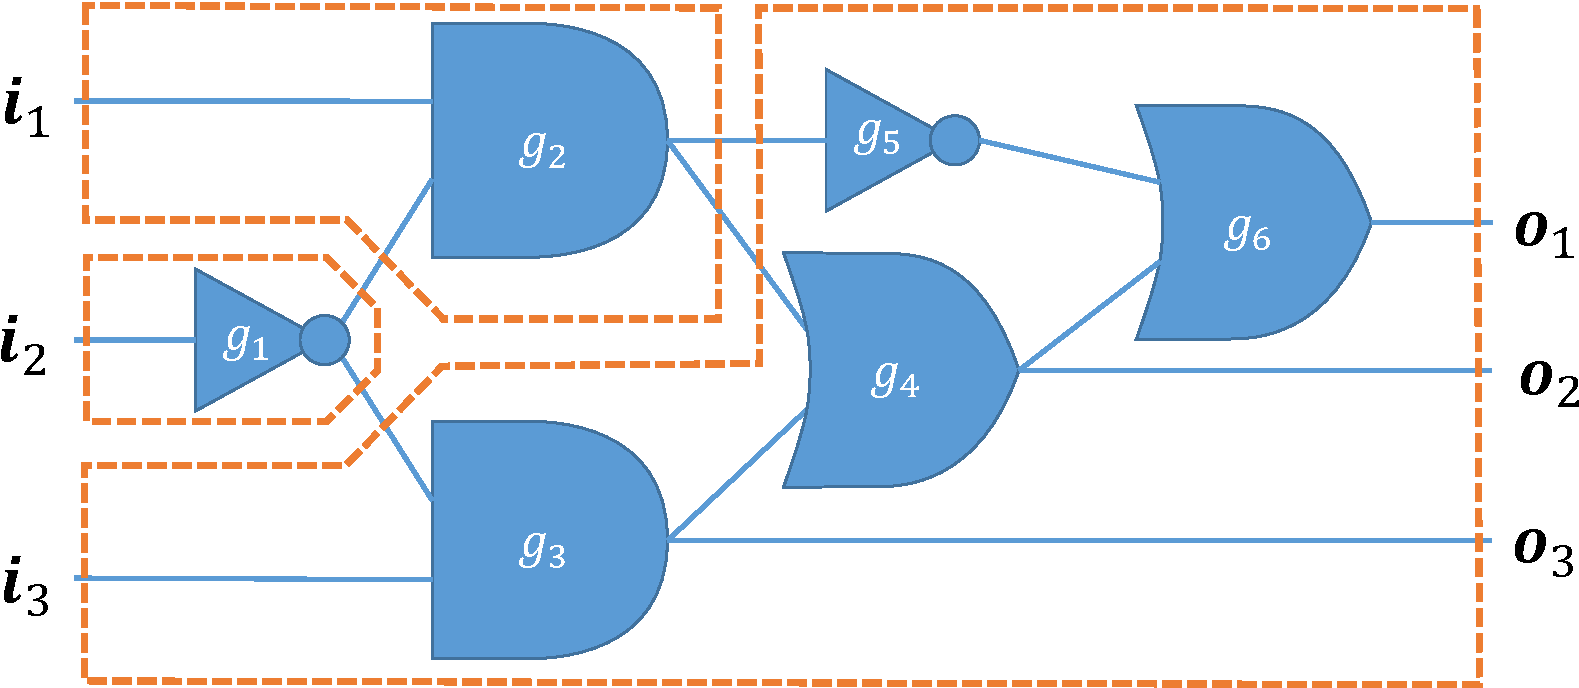
\includegraphics[height=60mm,clip]{img/fan-out-div.pdf}
  \end{center}
  \caption{図~\ref{fig:join} の回路を分割する例}
  \label{fig:fan-out-div}
\end{figure}
例えば,図~\ref{fig:join} の回路は,図~\ref{fig:fan-out-div} のように分割する.
$P({\bm i_2})$ を用いて $P(g_1)$ を表し,$P({\bm i_1}), P(g_1)$ を用いて $P(g_2)$ を表し,
$P(g_1), P(g_2), P({\bm i_3})$ を用いて $P({\bm o_1}), P({\bm o_2}), P({\bm o_3})$ を表す.
この時,数式は {\bf 補正ルール1} に従って生成される.
${\bm s}(0)$ の場合は,$P({\bm i_1}) = P({\bm i_2}) = P({\bm i_3}) = 0$ として計算し,
それ以外の要素についても同様に計算することで,正確な結果を求めることができる.

\chapter{実験結果}\label{chap:experiment}
\section{一般のシナリオ向けの実験}
\subsection{2x2行列の分解}
\subsection{4x4行列の分解}
\section{Selingerらの手法への適用シナリオ向けの実験}

\chapter{おわりに}\label{sec:conclusion}

% 本論文の概要と特徴
%In this work, we proposed the method to analyze the reliability of logic circuits.
%This method is efficient in memory usage by using directed acyclic graphs,
%and furthermore, Gray Code improves the execution time.
本研究では,組み合わせ回路における信頼性の評価方法について提案した.
提案手法は,無閉路有向グラフの利用によって,メモリの使用量を削減し,
グレイコードによって計算時間の面でも効率化を行った.
ただし,回路内に再収斂が存在する場合,この手法では正確な確率を計算することはできない.
そこでさらに,数式として計算し補正する手法と,そのための数式処理システムを提案した.

% 得られた成果
%The method does not calculate the correct probabilities if the circuit has the recomputation.
%However, this reconvergence do not heavily affect the results.
%According to our experiment,
%the memory usage is less than a ten-thousandth in the best case compared to the existing method
%and the calculated probabilities have accuracy within about 10\%.
実験結果の結果,数値として計算を行う提案手法は,
Probabilistic Transfer Matrix (PTM) を用いた既存手法に比べて,
メモリの使用量を 2 万分の 1 に抑えられるケースも存在する.
また,再収斂による誤差は,シミュレーションとの比較によれば,ほとんどのケースで 10\% 以内に抑えられた.
したがって,信頼性の評価に対して極めて深刻な誤差が発生するとは限らない.

% それから得られる最終結論

%このヒューリスティクスは、再集連を含まない場合に限り、正確な答えを出す。
%提案手法は、既存の厳密解を得る手法と比べてメモリの面で効率的であり、
%既存の入力パターンのサンプリングを行う場合と違い、
%全ての入力パターンに対して評価を行うことができる。
%あるいは、このヒューリスティクスに対して、
%さらに入力のサンプリングを行うことも可能である。

% 残された課題

既存手法では,指数的に増加する計算時間に対処するために,
いくつかの入力をサンプリングしたヒューリスティクスも開発されている.
提案手法についても,同様のヒューリスティクスが考えられる.
このとき,\ref{sec:prop:deform:reuse} を考慮すると,グレイコードによって,
1 ビット違いの連続した入力をサンプリングした方が効率が良い.
しかし,このサンプリング方法は,ランダムな入力を用いた場合に比べて偏りが生じるかもしれない.
サンプリングの方法によって,どの程度の偏りが生じるかは,検討すべき課題である.

提案手法は,メモリの使用量を削減したことで,分散コンピューティングにも容易に応用できる.
並列計算は,一般的にデータの転送時間がボトルネックとなりやすい.
しかし,提案手法の計算を入力パターンで分割し,ぞれぞれの入力パターンについて同時に計算する手法を考えると,
グラフ構造や数式のデータ構造を,各ユニットへ配布するだけでベクトル ${\bm s}$ を計算することができる.
さらに,${\it fidelity}$ の $l_1$-ノルムは,いわゆる並列リダクションで処理できる.
したがって,式~(\ref{eq:deformed}) の ${\bm v} \cdot {\bm s}$ の計算は,
MapReduce~\cite{mapreduce} と呼ばれるプログラミングモデルを適用することができると言える.
ベクトル ${\bm s}$ の計算と,ベクトル ${\bm v}$ との各要素同士の積を求めるまでが Map 操作に相当し,
それらの合計を求めるのが Reduce 操作に相当する.
分散コンピューティングで成功したモデルの一つである MapReduce との組み合わせによって,
設計時における信頼性の計算はさらなる高速化が期待できる.

%今後の課題としては、速度と正確性の改善である。
%The future study will focus on the speed and accuracy.
%Using a hash table of the sub-circuits may accelerate this method.
%By dividing a whole circuit and recomposing, we can omit the calculation of the same sub-circuit.
%Then the division and composition can solve the reconvergent problem
%when the input side of the sub-circuits do not contains many reconvergence.
%In addition, the accuracy of the results may rely on their topological distance.
%In that case, we may need to consider only gates near the reconvergent point to correct the error
%because it is anticipated that the effect of a distant reconvergent point would be trivial.


\chapter*{謝辞}

「このロボットを原発事故の現場に持っていくことはできないんですか?」\par
「あぁ,それはね,電磁波や放射線の影響で誤作動しちゃうんだよ…」\\
何年か前のうろ覚えな記憶ではありますが,RoboCup Japan Open の会場でこのような会話を耳にしました.
こうしてソフトエラーをテーマにした修士論文を書いてから思い返すと,
僅かながら運命的なつながりを感じる部分があります.
本研究のきっかけを与え,多大なるご指導をして頂きました,
立命館大学 情報理工学部 山下茂教授に深く感謝しお礼申し上げます.

次世代コンピューティング研究室の皆様に深く感謝申し上げます.
ユニークなイベントの数々は,他では味わえない貴重な経験になりました.
あらゆる立場から接していただき,将来の人生を豊かにするための様々なヒント得ることができたと思います.
共に過した多くの時間は,決して忘れることないでしょう.

情報理工学部プロジェクト団体や,立命館大学コンピュータクラブの皆様にもお礼申し上げます.
志の高い先輩や後輩,そして同期の方々に出会い,
成長の機会と経験を得ることができました.
今後とも活躍を期待し,応援したいと思います.

最後に,大学生活を支えていただき,育てていただいた両親にお礼申し上げます.


\bibliographystyle{junsrt}
\bibliography{references}
\end{document}

